\subsection{The Google File System}
The Google File System (GFS) \cite{DBLP:conf/sosp/GhemawatGL03} is the distributed file-system employed internally by Google until it was replaced by Colossus, another internal system (which remains unpublished at the time of this writing). 
The design of GFS and MapReduce \cite{DBLP:journals/cacm/DeanG08} directly drove the implementation of the Hadoop platform and, as such, there are many similarities between GFS and HDFS.

\subsubsection{Architecture}
\begin{figure}[h]
\caption{GFS architecture diagram}
\label{fig:gfs-architecture}
\centering
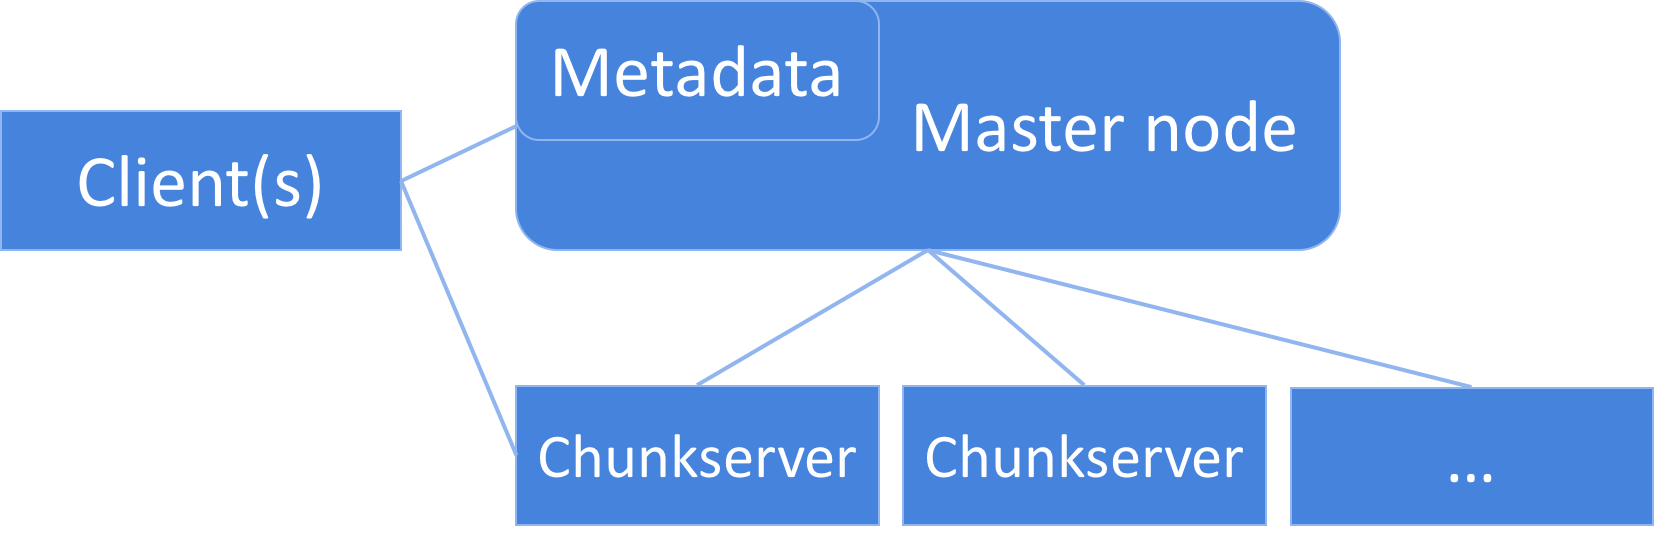
\includegraphics[width=1.0\textwidth]{images/gfs-block-diagram.png}
\end{figure}

GFS is designed as a distributed non-POSIX-compliant file-system for distributed applications and it is built by clustering a set of general-purpose machines as shown in Figure \ref{fig:gfs-architecture}.
It is a distributed system with three distinct roles: 
\begin{itemize}
    \item a \emph{master node}, which maintains metadata on files and the state of the system,
    \item a set of \emph{chunkservers} which perform storage of data on disk and directly interact with clients, and
    \item clients which read and write data from/to the system.
\end{itemize}
In the system files are divided in chunks, which can grow up to 64 megabytes before another chunk is created.
The master stores both the hierarchy of files and directories, as well as information on which chunks form any given file.
Multiple copies of each chunk (three by default), referred to as replicas, are managed by different chunckservers operating in different failure domains.
Chunks are stored as regular files in the chunkserver's local filesystem.
Replication is employed to maintain data availability in the face of chunckserver failure, as well as to provide a limited form of load balancing by allowing different clients to read different replicas of the same block.
The location of replicas is stored, alongside all other file metadata, in the master main memory.

As in HDFS, the single master node is the main scalability and reliability bottleneck for the system and, as such, many techniques employed in GFS have to goal of reducing interactions with this node to a minimum and increase its reliability.
\paragraph{Reads} The chunk size is purposefully very large compared to local file-systems, as any read request must first contact the master to learn the location of block replicas.
When responding to such a query, the master sends location data about several following blocks in the file and this information is cached by clients for a short period of time, to avoid excessive master involvement in sequential read scenarios.
After learning the location of blocks, the client can complete the read operation with no further involvement from the master node, by contacting the relevant chunkservers directly.
\paragraph{Writes} In order to minimize the master's involvement in write operation, the systems grants block leases to chunckservers.
When a client requests to mutate a block, either by writing or appending to it, the master selects three (assuming a default replication factor) chunkservers to receive the mutation: a \emph{primary} and two replicas.
The primary is granted a new lease to alter a block with data received by the client for as long as the lease is valid, unless it was already holding a lease for the specified block.
The chunckserver can periodically renew the lease by contacting the master node if it is still receiving data from clients.
At this point, the client pushes the data to all the chunkservers and waits for a confirmation that all of the replicas received the data.
When a confirmation is received the client contacts the primary and requires a write operation.
The primary serializes all writes (there may have been concurrent writes) and then applies them to the file stored on the local disk.
After it applied the state to the local file it contacts the replicas and asks them to write the changes in the same order.
Once it receives confirmation from all replicas, the write is finally acknowledged to the client.
\paragraph{Reliability} In order to increase the master reliability, all metadata mutations are persisted on a disk-based log which is both kept on the local machine and replicated to a number of others.
Client operations that involve metadata modifications are not acknowledged before this flush is completed.
Given that such a mutation log would grow without bounds, it is periodically compacted into a snapshot.
The snapshot is created by serializing the current master metadata on disk in a format that can be directly used to restore a master without any parsing.
When a master needs to recover from a crash, first it loads the most recent snapshot, then it applies all the modifications in the log before accepting any client queries.
This mutation log is also used to keep several ``shadow masters'' up-to-date with the state of the master.
Shadow masters cannot perform any metadata mutation but they can serve read requests, even in the event of master failure.
This mechanism is used both to scale the system further by delegating reads to a shadow master and to grant a read-only service during recovery of the master.

\subsubsection{Chunk management}
While client-initiated operations are optimized to involve the master infrequently, some periodic operations are necessary to keep the cluster in a healthy state.
As previously mentioned, GFS uses replication to maintain data availability in the face of chunkserver failure.
However, if chunks with fewer than three replicas are not replaced, eventually all replicas will be unavailable.
To prevent this, the master periodically queries all chunkservers for the list of all chunks they are holding and instructs the chunkservers to re-replicate the ones with fewer than the specified number of replicas (three by default).
Finally, chunk deletion is also handled asynchronously, if the master detects any chunks that are not tracked in its memory metadata, the corresponding chunkserver is instructed to delete the chunk from disk.